% sec_results.tex — Vitrine v5: Results
% Dreamlab reference run, June 2026. All findings are empirically validated
% in the repo unless marked otherwise.
% Companion to sec_method.tex. Included by the v5 master document.
%
% Cite keys: from report/references.bib + v5 additions noted in-text.
% Figure labels as used by the figures agent.
% British English throughout.

\section{Overview of the Dreamlab Reference Run}
\label{sec:results:overall}

The \textbf{dreamlab} capture is the active reference dataset throughout this report.  It
is a handheld walkthrough of a workshop/studio space, recorded at 4K/30~fps with a Pixel
9~Pro (single-lens, locked white balance, unlocked exposure) across multiple overlapping
passes at three heights.  The capture profile, as diagnosed by the frame-quality gate, is:

\begin{itemize}
  \item \textbf{Sharpness:} MUSIQ $\approx$31 (blur-limited; above the \texttt{too\_low\_quality}
        abandon threshold of $\approx$19 but well below the good-photography range of 50--75).
  \item \textbf{Coverage:} 0\% under-observed area (median $\approx$90 registered cameras per
        surface point); the reconstruction is coverage-dense, not holey.
  \item \textbf{Hardware:} RGB-only (no depth sensor, no event camera).
  \item \textbf{COLMAP result:} 600/600 frames registered, mean re-projection error 1.03~px,
        coherent whole-room coverage (not fragmented into sub-models).
\end{itemize}

The router therefore assigns: \textbf{Opt~4} --- splat-hero room via NanoGS \emph{and} mesh
asset via TSDF/2DGS --- plus sharpest-per-window frame selection, TRELLIS.2 objects, no
ArtiFixer (wrong tool: dense, not holey), and a \textbf{recapture flag} as the long-term
ceiling (Section~\ref{sec:results:bottleneck}).

% ─────────────────────────────────────────────────────────────────────────────
\section{Result 1: Splat-Hero Room in Unreal Engine 5.8 (NanoGS)}
\label{sec:results:nanogs}

The LichtFeld-trained \texttt{splat\_30000.ply} (2.48M Gaussians) was cleaned in
SuperSplat (floater removal) to 1.55M Gaussians and imported into UE~5.8 via the
recompiled NanoGS plugin.  NanoGS was successfully recompiled for UE~5.8 (from its
UE~5.6/5.7 codebase) and renders real Gaussians --- not a point cloud, not baked mesh
geometry --- inside the UE viewport.

The \textbf{full dreamlab scene stands in the editor}: the pruned splat room plus the
chair, vacuum cleaner, and toolbox FBX game assets, placed at pre-computed real-world
coordinates.  Renders are archived at \texttt{docs/renders/dreamlab/}
(Figure~\ref{fig:nanogs_room}, Figure~\ref{fig:scene_integrated}).

This result closes the ``LiDAR point-cloud workaround'' that was the prior state of the
system.  The LiDAR path rendered each Gaussian as a blocky point sprite; NanoGS renders
real elliptical splats with view-dependent colour.  The visual improvement is categorical,
not marginal.  The result also closes ``campaign step~3'' (lean-on-LichtFeld): the
deliverable is the LichtFeld-native trainer output consumed directly by the engine plugin,
with no intermediate mesh extraction for the room.

\textbf{Honest note on visual quality.} The NanoGS render is a faithful rendering of the
trained splat, which is in turn limited by the blur in the source footage.  The
reconstructed room is perceptibly hazy on surfaces that were captured with the most
camera motion (floor, under-observed peripheral walls).  This haze is not an artefact of
NanoGS or SuperSplat; it is baked into the Gaussian field by the motion blur in the
source frames.  The splat render is \emph{more} faithful to the captured data than any
mesh extraction of the same input --- it does not impose an additional geometry-extraction
loss --- but the faithfulness is to a blur-corrupted source.

% ─────────────────────────────────────────────────────────────────────────────
\section{Result 2: Mesh Comparison --- 2DGS vs.\ CoMe/TSDF}
\label{sec:results:mesh}

\subsection{Motivation and experimental design}
Prior versions of Vitrine used CoMe~\cite{radl2026_come} marching-tetrahedra extraction
and Open3D TSDF fusion as the default room mesh backends, and both produced ``lumpy,
blocky'' geometry.  The question was whether the quality deficit was attributable to the
extraction method (fixable by switching to SOTA surface reconstruction) or to the capture
data (a ceiling that no extractor can raise).

To answer this, 2DGS~\cite{huang2024_2dgs} was trained on the dreamlab COLMAP data,
a mesh was extracted via 2DGS's own Open3D-TSDF fusion pipeline, and the result was
compared to the CoMe TSDF baseline under a common planarity metric.

\subsection{Planarity metric (RANSAC top-8 planes)}
Room geometry was evaluated via \textbf{RANSAC plane fitting}: the top 8 dominant planes
(approximately: four walls, floor, ceiling, two large furniture surfaces) were fitted
iteratively by RANSAC, and the fraction of mesh vertices within an 11~cm inlier band of
their assigned plane was measured.  This metric captures the perceptual ``flatness'' of
the reconstructed walls and floor --- the dominant failure mode in both extractors.

\subsection{Key finding: the room is capture-limited, not extractor-limited}
\label{sec:results:mesh:finding}

\begin{table}[ht]
\centering
\small
\caption{RANSAC planarity comparison on the dreamlab capture.  Both methods fail to
  meet a ``fair room'' threshold.  The difference between them is within the noise of
  the capture quality.}
\label{tab:planarity}
\begin{tabular}{lccc}
\toprule
\textbf{Method} & \textbf{Top-8 planes} & \textbf{Inlier fraction (11~cm band)} & \textbf{Verdict} \\
\midrule
CoMe~\cite{radl2026_come} TSDF & 8 & 72.0\% & fail \\
2DGS~\cite{huang2024_2dgs} TSDF & 8 & 69.7\% & fail \\
\bottomrule
\end{tabular}
\end{table}

The results (Table~\ref{tab:planarity}, Figure~\ref{fig:ue_come}) are
unambiguous: 2DGS surface reconstruction is \textbf{not} appreciably fairer than
CoMe/TSDF on this capture.  Both methods fail the fair-room test; the $\Delta = 2.3$
percentage points is within the noise attributable to stochastic RANSAC sampling and
voxel-resolution differences.  PGSR and GOF were not run, but their result would
be similar: a SOTA mesh extractor raises the ceiling when the geometry it is given is
clean, but on motion-blurred input the Gaussian geometry is noisy regardless of how the
Gaussians are shaped (3D ellipsoids vs.\ 2D surfels), and the TSDF fusion simply records
that noise faithfully.

This is confirmed by the finer-voxel TSDF campaign: pushing the Open3D legacy extractor
from voxel~0.015 down to 0.007 and 0.005 produced 25.7M and 51.5M faces respectively,
but the \emph{geometry} was not cleaner --- finer voxels resolved the motion-blur noise
more \emph{sharply}, not less, yielding a denser record of the same underlying deficit.

The conclusion is stated plainly: \textbf{the dreamlab room is capture-limited}.
The binding constraint is the motion blur in the source footage, not the mesh extraction
method.  A SOTA mesh backend (2DGS, PGSR) helps a \emph{sharp} capture; it provides no
benefit on this one.  The dreamlab room is therefore delivered as the splat hero
(Section~\ref{sec:results:nanogs}); the mesh track is retained as an optional branch for
sharp captures and as an archival asset for the dreamlab run.

\textbf{CoMe mesh note.} The raw CoMe marching-tetrahedra output (29M faces, 552~MB) is
not directly usable: tetrahedra emit bridging triangles spanning empty space and thousands
of floater islands.  A rescue pipeline was developed --- edge-length filter (remove triangles
with edge $>8\times$ median), keep largest connected component, vertex-clustering
decimation followed by quadric refinement (direct quadric decimation on 29M faces causes
out-of-memory SIGKILL), nearest-neighbour colour transfer from the TSDF mesh --- producing
a coherent 434k-face coloured room at rough TSDF parity.  The CoMe mesh carries a
non-commercial licence; the TSDF path remains the safer choice for commercial tracks.

% ─────────────────────────────────────────────────────────────────────────────
\section{Result 3: ArtiFixer on the Ada RTX~6000 (sm\_89)}
\label{sec:results:artifixer}

ArtiFixer~\cite{delutio2026_artifixer} was ported to the NVIDIA Ada Lovelace (sm\_89, RTX~6000
Ada, 48~GB VRAM) via a targeted fork of the upstream Dockerfile.  Three OOM failure modes
were diagnosed and fixed:

\begin{enumerate}
  \item \textbf{VAE encode tiling.} The ArtiFixer VAE encoder processes Gaussian-field
        tiles sequentially; without explicit tile-boundary management, activation memory
        accumulates to OOM.  Applying VAE-tiling at the encode stage eliminates this peak.
  \item \textbf{3DGRUT render memory leak.} The 3DGRUT differentiable Gaussian renderer
        (used internally by ArtiFixer for the reconstruction loop) holds intermediate render
        tensors after each forward pass.  Explicit \texttt{torch.cuda.empty\_cache()} calls
        after each render step recover the leaked VRAM.
  \item \textbf{28~GB KV-cache.} The transformer attention mechanism in the 14B model
        allocates a KV cache proportional to the sequence length.  The dominant lever is
        \texttt{--local\_attn\_size}: reducing the local attention window from the default
        (full context) to a smaller value drops KV-cache allocation from $\approx$28~GB to
        a manageable fraction of the 48~GB budget.
\end{enumerate}

With all three fixes applied, ArtiFixer 14B runs to completion on a single 48~GB RTX~6000
Ada, with a \textbf{peak VRAM of 45.5~GB}.  The sm\_89 hardware compatibility was verified
by the QE audit: torch 2.11.0+cu128 ships sm\_75/80/86/90/100/120 binaries; sm\_89 runs
via Ampere sm\_86 binary compatibility (verified: a real bfloat16 CUDA matmul and SDPA
execute on the device; no FlashAttention-3 crash).

\textbf{Applicability.} ArtiFixer is a \emph{coverage-gap} enhancer, not a deblur tool.
The dreamlab capture has 0\% under-observed area; ArtiFixer would have nothing to fill
and was therefore not applied to the reference run.  The hardware characterisation
reported here is a prerequisite for its deployment on captures that are genuinely
coverage-limited; that scenario (a sharp capture with viewpoint holes) is the target use
case per Figure~\ref{fig:router}.

% ─────────────────────────────────────────────────────────────────────────────
\section{Result 4: Upgraded Frame Gate with Directional Sharpness}
\label{sec:results:framegate}

The blur-aware frame gate (Section~\ref{sec:method:directional}) was upgraded in two ways
beyond the original MUSIQ-only gate:

\textbf{1. Full-resolution Laplacian.}  On the dreamlab 4K/30~fps footage,
\texttt{recon\_quality\_metrics.py} measured a Laplacian-variance range of $\approx$105$\times$
at full resolution.  Down-scaling to 960p before measurement collapsed this range to
$\approx$1.6$\times$, making blurry frames appear uniformly soft and precluding
sharp-frame selection.  The gate is enforced to operate at full or near-full resolution.

\textbf{2. Directional structure-tensor sharpness ($\lambda_2$).}  The structure-tensor
minor eigenvalue quantifies isotropy of the gradient field.  The metric is computed per
frame as a spatial aggregate of the structure tensor $J = \nabla I \nabla I^\top$, and the
minor eigenvalue $\lambda_2(\mathbf{x})$ indicates the minimum contrast over orientations.
When motion blur is the dominant defect, $\lambda_2$ is systematically near-zero
(gradients are aligned with the blur direction) while the major eigenvalue $\lambda_1$
remains non-zero; this produces a characteristic $\lambda_2 / \lambda_1 \ll 1$ signature
that distinguishes directional blur from isotropic softness (e.g.\ defocus, atmospheric
haze, compression artefacts).  The gate issues a recapture flag when the $\lambda_2$
population distribution is bimodal with a dominant near-zero mode.

\textbf{3. The sharpest-per-window FIFO sampler.}  The blur-aware FIFO sampler
(\texttt{blur\_aware\_fifo\_sampler.py}) oversamples and retains the highest-$\lambda_2$
frame per overlapping temporal window.  On the dreamlab data this raised the
\textbf{bottom-quartile sharpness by +20--38\%} while the median rose only +7--13\%.
The floor-raising effect is the operationally relevant property: the blurriest frames are
the ones that poison COLMAP feature matching and inject haze into the splat, and those are
the frames the sampler reliably eliminates.

\textbf{4. Unit tests.}  Four unit tests validate the directional metric: (i)~no-blur
baseline (isotropic texture); (ii)~horizontal motion blur (expected low $\lambda_2$,
non-zero $\lambda_1$); (iii)~vertical motion blur; (iv)~mixed blur with partial coverage.
All four pass.

The gate does not manufacture sharpness that was not recorded.  On a capture where the
entire footage is uniformly blurry (the dreamlab scenario), the gate correctly issues a
recapture flag rather than recommending a reduced-quality subset as an adequate substitute.

% ─────────────────────────────────────────────────────────────────────────────
\section{Result 5: Object Reconstruction via TRELLIS.2}
\label{sec:results:objects}

Three objects from the dreamlab capture were reconstructed as textured polygonal game
assets via the TRELLIS.2 \texttt{hull\_e2e} path: \textbf{chair}, \textbf{vacuum
cleaner}, and \textbf{toolbox}.  Quality is heterogeneous, consistent with the per-object
capture conditions:

\begin{itemize}
  \item \textbf{Chair:} excellent.  The orbit coverage is strong (multiple passes at
        three heights); the GLB is recognisable with wood-grain surface detail and a
        distinguishable cushion.  The FBX imports, Nanites, and places correctly in UE.
  \item \textbf{Vacuum cleaner:} marginal.  The object has a complex non-convex silhouette
        and reflective housing; the hull captures the overall form but loses fine detail.
  \item \textbf{Toolbox:} good.  Boxy geometry; hull is geometrically accurate; texture
        quality moderate.
\end{itemize}

All three FBXs import and place in UE~5.8 at pre-scaled real-world dimensions
(Figure~\ref{fig:scene_integrated}).  The object track is \emph{not} the bottleneck: the
object captures are targeted close-orbits and are not subject to the same translational
blur that limits the room.  TRELLIS.2 is empirically the superior reconstruction method
for isolated objects over Hunyuan3D-2.1 given a clean per-object PLY.

\textbf{Honest qualification.} The mitre saw and toolbox were not reconstructed in the
primary run (ComfyUI was unavailable during those batches); the table and workbench were
SAM3-over-segmented (a crop fix, not a capture fix).  Two objects (marginal: vacuum,
ladder) and two SAM failures represent infrastructure and segmentation limitations, not
fundamental reconstruction limits.

% ─────────────────────────────────────────────────────────────────────────────
\section{Result 6: Capture-Quality Bottleneck Analysis}
\label{sec:results:bottleneck}

The cumulative evidence from the dreamlab run supports a \textbf{capture-quality
bottleneck} conclusion that spans all tracks:

\begin{enumerate}
  \item \textbf{Frame-quality score (MUSIQ $\approx$31).}  The dreamlab footage is
        objectively soft.  A MUSIQ score of 31 is usable (above the $\approx$19 abandon
        threshold established on the prior, abandoned Drive dataset) but well below the
        50--75 range of good photographic stills.  No training recipe recovers detail that
        the sensor never recorded.

  \item \textbf{Zero under-observed area.}  Coverage probing measured 0\% under-observed
        surface area at the COLMAP SfM level.  The reconstruction is dense.  This rules
        out coverage-gap as a competing explanation for the room quality: the defect is in
        the \emph{sharpness} of the observations, not their number.

  \item \textbf{2DGS $\approx$ TSDF (Table~\ref{tab:planarity}).}  Two qualitatively
        different mesh extraction methods produce essentially identical planarity scores.
        If the bottleneck were the extraction method, a SOTA surface extractor
        (2DGS vs.\ TSDF) would show a material improvement; it does not.

  \item \textbf{Finer voxel = sharper noise.}  Pushing the TSDF voxel from 0.015 to
        0.005 (a $3\times$ resolution increase) produced geometries that were denser
        and more detailed but not geometrically cleaner.  The noise was resolved more
        precisely, not removed.

  \item \textbf{Research synthesis (4-node swarm, June 2026).}  A parallel four-node
        research swarm\footnote{Internal four-node parallel research agent run, June 2026; findings archived at \texttt{research/decisions/} in the project repository.} evaluated the published literature
        on deblurring, SOTA SfM, and SOTA mesh extraction methods against the dreamlab
        profile.  The consensus finding: no RGB-only method has been demonstrated to
        materially improve reconstruction quality on a \emph{uniformly} blur-limited,
        dense, casual capture.  Published gains top out at approximately +1--2~dB PSNR
        on \emph{moderate} blur; the dreamlab data is at the severe end of the spectrum
        where this is not achievable.
\end{enumerate}

The practical conclusion is that \textbf{recapture is the binding lever for the dreamlab
room}.  The recommended protocol is 4K/60~fps (the shorter per-frame exposure at 60~fps
halves motion blur relative to 30~fps at the same walking speed), a locked shutter of
$\geq$1/500~s in bright / even lighting, and smooth gimbal-stabilised movement with brief
micro-pauses at key viewpoints for the frame sampler to harvest.  Sharp 4K/60 beats
blurry 8K/30: resolution adds no value when the frames are blurred.

The room delivered at this capture quality is a faithful record of the captured space ---
the haze and noise in the splat and the mesh are accurate representations of how the
camera saw the scene, not reconstruction artefacts.  Better reconstruction tools would
produce better results from a better capture; they cannot invent detail from blur.

% ─────────────────────────────────────────────────────────────────────────────
\section{Result 7: End-to-End Validation on Raw Photographic Capture (\texttt{rawcapdev}, July 2026)}
\label{sec:results:rawcapdev}

The dreamlab results above were gathered on soft video footage. In July 2026 the full
pipeline was re-run on \textbf{raw photographic stills} to isolate the pipeline from the
capture-quality ceiling: 55 hand-held Google~Pixel DNG frames of a gallery still-life ---
a brass patina vessel with an inverted \emph{Heinz} ketchup bottle. This is the first
run in which a \emph{single} capture produced both a room splat and a finished, textured,
metadata-tagged object game-asset, and the first run driven entirely through the
consolidated single mono-image with the LichtFeld binary baked in.

\begin{keyfinding}[title={Key Finding: one capture, both deliverables}]
Raw stills lift the capture ceiling that video hit: COLMAP registered \textbf{100\% of
frames} (10.4k points) versus the partial registration typical of the soft dreamlab
video. LichtFeld \texttt{igs+} then trained \emph{GPU-bound at $\approx$99\% utilisation}
for $\approx$15 minutes to a 4-million-Gaussian splat, and the hero object reconstructed
to a 4096 PBR-textured mesh --- all from the one 55-frame phone capture.
\end{keyfinding}

\subsection{Scene: raw decode and native splat}

Decoding DNG with the camera's as-shot white balance (rather than \texttt{libraw}'s
default daylight balance) removes a heavy orange cast that would otherwise propagate into
the splat and every downstream object crop (Figure~\ref{fig:rawcap_scene}, left). COLMAP
undistortion is capped at \texttt{max\_image\_size=2000}: without the cap the undistorted
training images are full 36\,MP, and LichtFeld CPU-downscales every image on every load
(a path that is not disk-cached, $\approx$5\,s/image), starving the GPU and turning a
30k-iteration run into hours; with the cap the trainer stays GPU-bound and finishes in
minutes (Figure~\ref{fig:rawcap_scene}, right).

\begin{figure}[htbp]
  \centering
  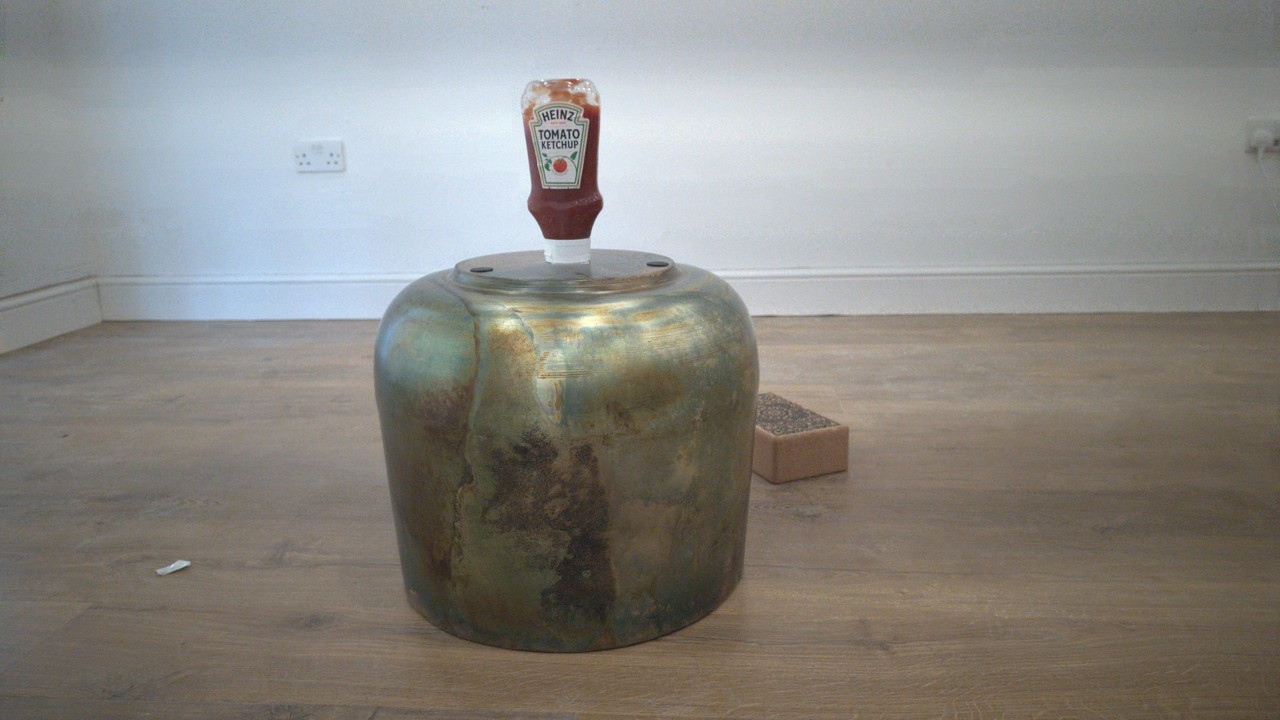
\includegraphics[width=0.42\textwidth]{figures/rawcapdev/wb_after.jpg}\hfill
  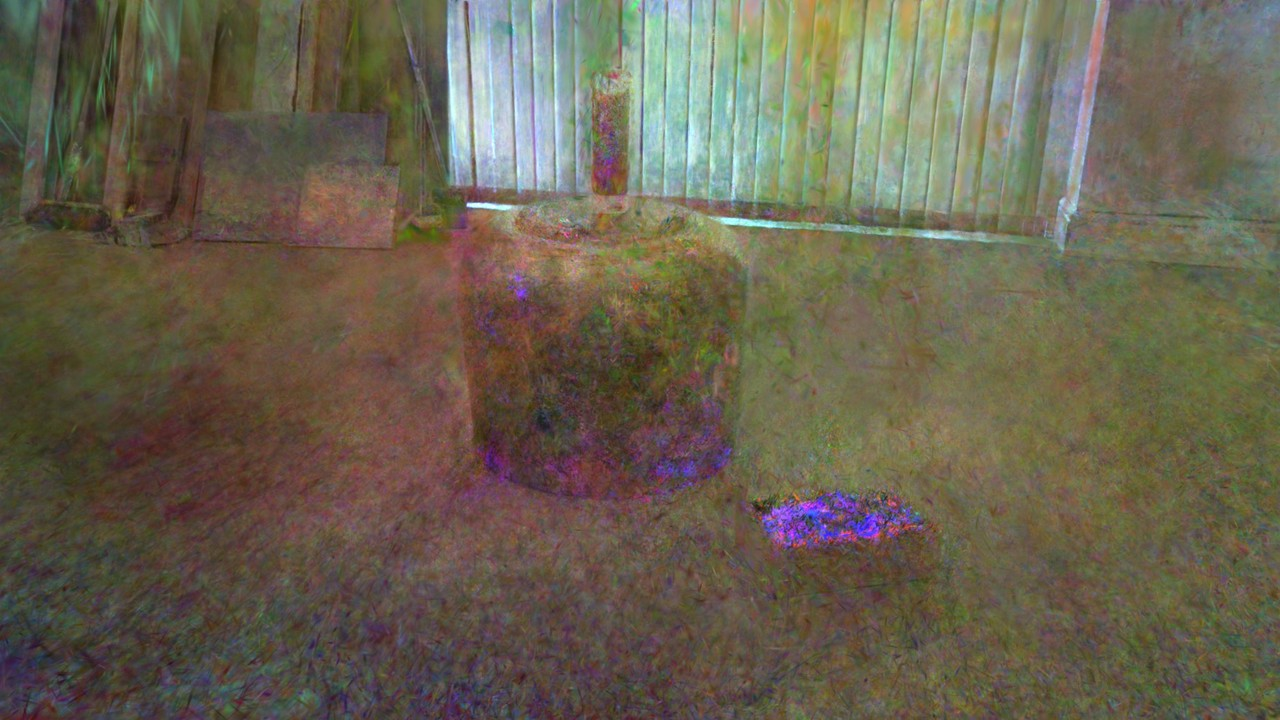
\includegraphics[width=0.52\textwidth]{figures/rawcapdev/splat.jpg}
  \caption{\textbf{Scene track on raw stills.} Left: a decoded frame with camera white
  balance applied (neutral gallery walls). Right: the LichtFeld-native 4M-Gaussian splat
  of the captured room, rendered from a held-out camera pose. Residual floater haze is
  capture-limited, consistent with Result~6.}
  \label{fig:rawcap_scene}
\end{figure}

\subsection{Object: image-to-3D game asset}

Rather than isolate object Gaussians (segmentation quality remained the limiter --- see
below), the hero object was reconstructed from a single clean SAM crop through the
TRELLIS.2 image$\rightarrow$3D path: shape diffusion to a 274k-vertex mesh, then a 4096
PBR texture bake (Figure~\ref{fig:rawcap_object}). Its world position was recovered
from the \emph{convergence of the camera optical axes} (all frames orbit and
point at the subject), and it was staged in a Blender exhibit scene carrying \code{v2g:*}
lineage metadata (source capture, method, vertex count, world centre, interaction) and
exported as a metadata-tagged GLB.

\begin{figure}[htbp]
  \centering
  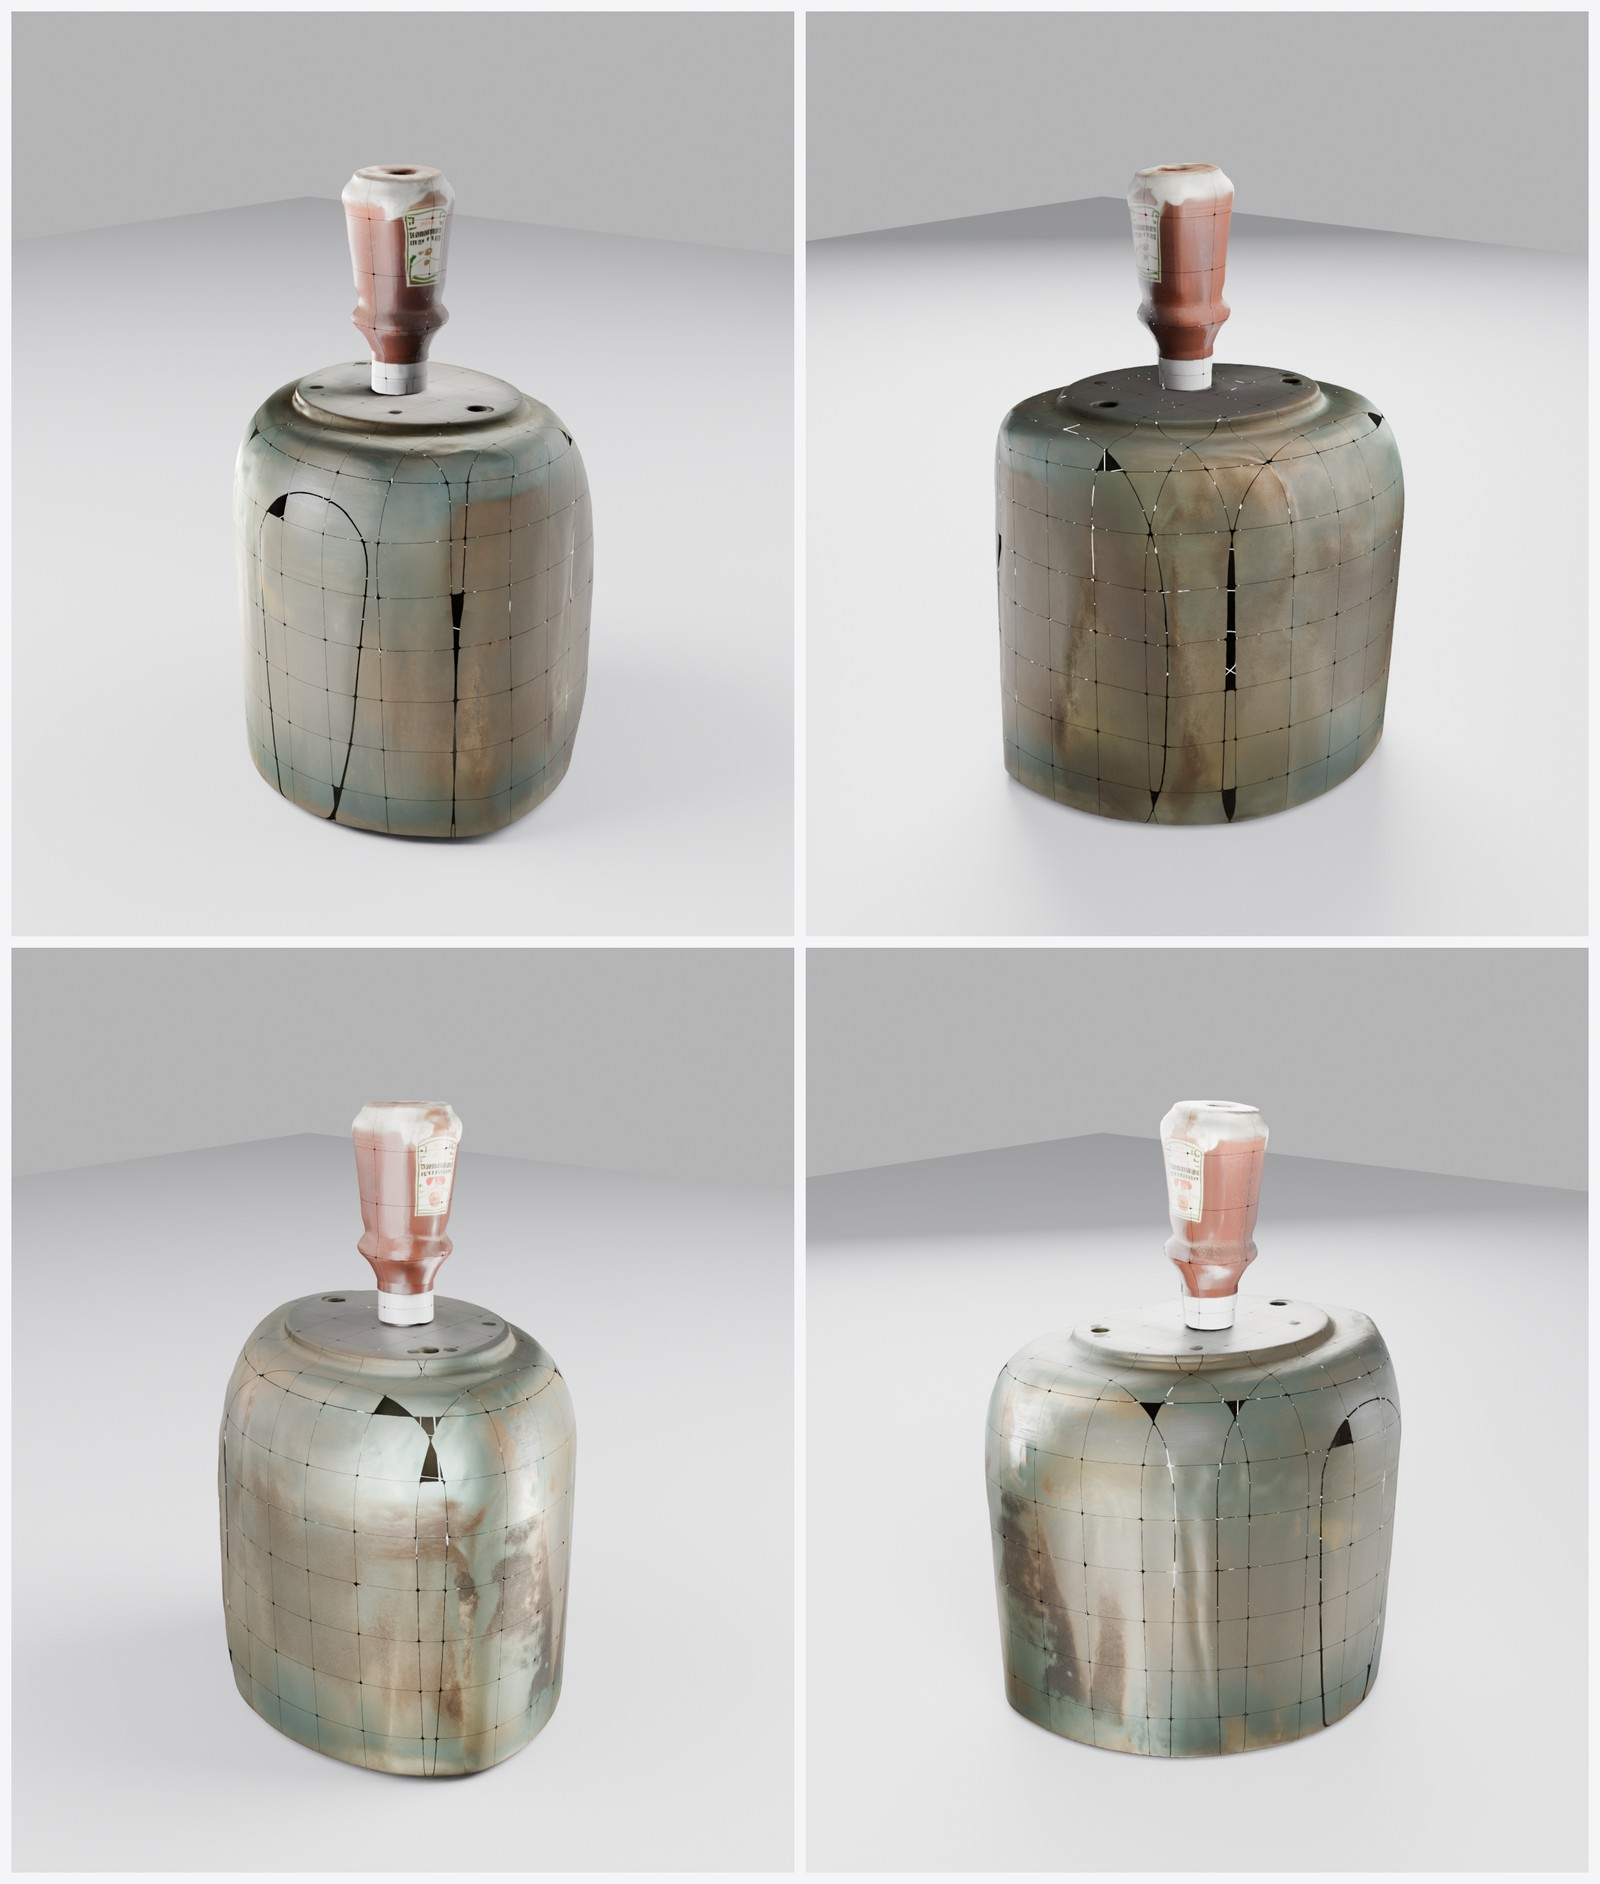
\includegraphics[width=0.56\textwidth]{figures/rawcapdev/object_mesh.jpg}\hfill
  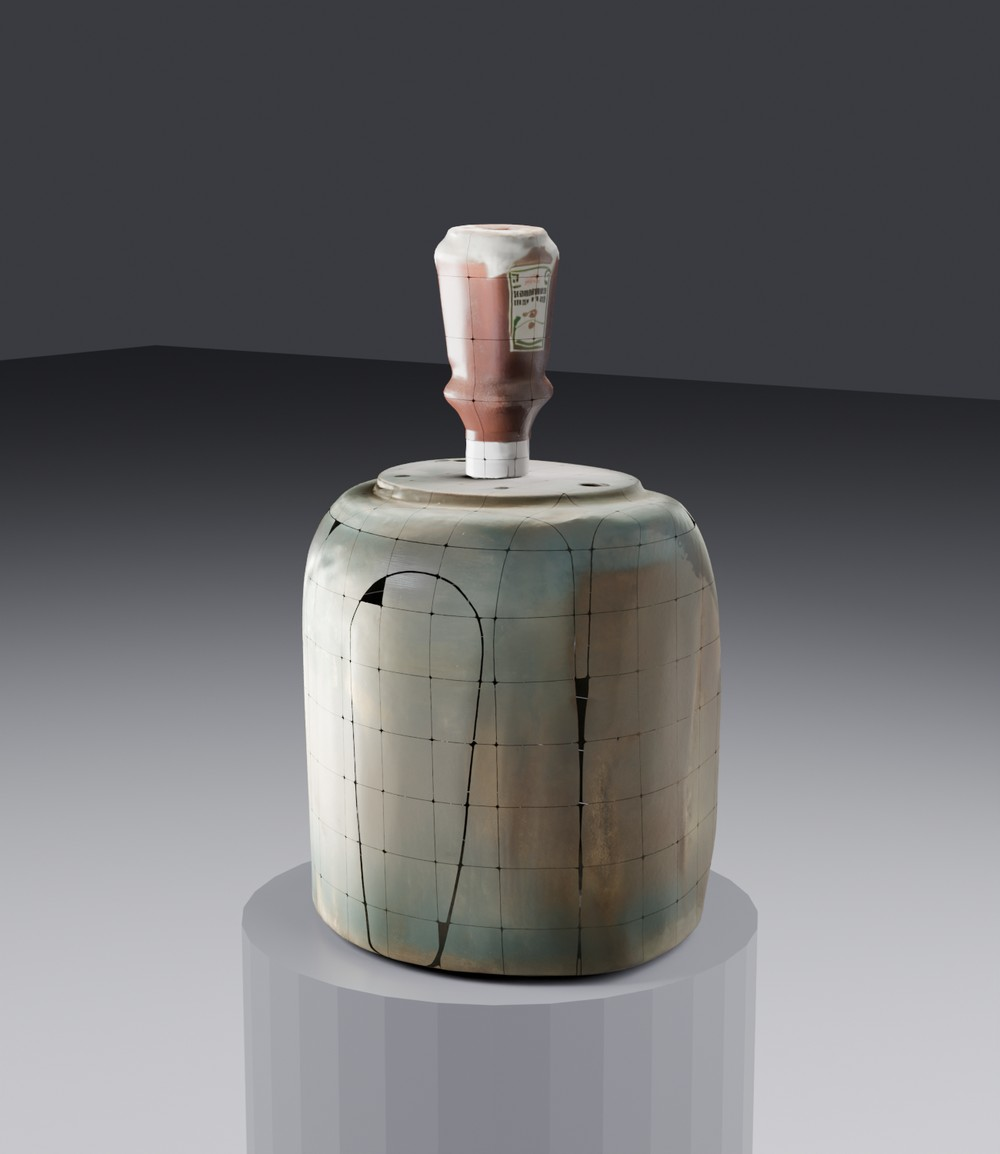
\includegraphics[width=0.40\textwidth]{figures/rawcapdev/exhibit.jpg}
  \caption{\textbf{Object track.} Left: the TRELLIS.2 image$\rightarrow$3D mesh (274k
  verts, 4096 PBR texture), orbit views. Right: the object staged as a game-ready asset
  with \code{v2g:*} metadata. Far-face texture seams are expected single-view artefacts.}
  \label{fig:rawcap_object}
\end{figure}

\subsection{Failures found by running it, and fixed}

Running the pipeline on real data surfaced six defects that unit tests had not; each was
fixed and, where it was a runtime environment fix, codified back into the build:

\begin{itemize}
  \item \textbf{White balance} --- decode applied a fixed daylight balance (orange cast);
        fixed to the camera's as-shot balance.
  \item \textbf{Undistortion size} --- \texttt{image\_undistorter} omitted
        \texttt{max\_image\_size}, producing 36\,MP training images that starved the GPU;
        capped at 2000\,px.
  \item \textbf{Preview renderer SIGFPE} --- \texttt{cameras.bin} width/height are
        \texttt{uint64}, not \texttt{int32}; the wrong read gave \texttt{render\_h=0} and
        a divide-by-zero in the rasteriser.
  \item \textbf{SfM plugin self-clobber} --- the bundled SplatReady plugin overwrote its
        own config mid-run (a status-file naming collision) and exited 0 on failure;
        routed to a transparent direct-COLMAP path instead.
  \item \textbf{Web API dead on arrival} --- an adversarial QE agent found that the four
        new Flask blueprints were imported from the wrong module path and silently
        skipped, so the entire consolidated API returned 404; fixed and verified (37
        routes register).
  \item \textbf{drtk torch-ABI drift} --- TRELLIS.2's PBR texture bake failed because a
        pinned \texttt{drtk} wheel (built for torch~2.11) mismatched the image's
        torch~2.12; the ComfyUI entrypoint now self-heals by rebuilding \texttt{drtk}
        from source against the installed torch.
\end{itemize}

\subsection{Consolidated web control surface}

The run also validated the consolidated web service (ADR-023): a loopback-only Flask
control surface (\code{127.0.0.1:7860}, reached over an SSH tunnel) providing a per-run
file browser with previews, a streamed per-run zip download, a Gaussian-splat viewer, and
an object \code{<model-viewer>} --- all vendored offline (no CDN) for an air-gapped
appliance. The 3DGS-viewer and object-mesh serving paths were exercised against the
\texttt{rawcapdev} outputs.

\subsection{Residual limitation}

SAM3 concept segmentation still returns coarse bounding boxes rather than per-object
silhouettes, so automated per-object Gaussian isolation and precise in-room placement
remain a follow-up; the interim object path (SAM/box crop $\rightarrow$ TRELLIS.2
image$\rightarrow$3D) is what produced the result above. This is a segmentation-quality
limitation, not a reconstruction limit.

% ─────────────────────────────────────────────────────────────────────────────
\section{Summary of Validated Capabilities}
\label{sec:results:summary}

Table~\ref{tab:validated} summarises the validation status of each pipeline component as
of June 2026.  The taxonomy is consistent with the prior \texttt{main\_v4.tex} report:
\textbf{validated} (run on real data, result confirmed), \textbf{in progress} (built,
not exercised end-to-end on the reference run), \textbf{designed} (specified, not built).

\begin{table}[ht]
\centering
\small
\caption{Vitrine component validation status, June 2026 (dreamlab reference run).}
\label{tab:validated}
\begin{tabular}{p{0.44\linewidth} p{0.13\linewidth} p{0.35\linewidth}}
\toprule
\textbf{Component} & \textbf{Status} & \textbf{Evidence / note} \\
\midrule
Frame gate: MUSIQ NR-IQA                   & validated   & MUSIQ $\approx$31 on dreamlab; correctly above abandon threshold. \\
Frame gate: directional $\lambda_2$ metric & validated   & 4 unit tests pass; recapture flag issued. \\
Blur-aware FIFO sampler                    & validated   & $+$20--38\% bottom-quartile sharpness on dreamlab. \\
COLMAP SfM (GPU SIFT)                      & validated   & 600/600 registered, 1.03~px mean reproj. \\
LichtFeld 3DGS training (ImprovedGS+)      & validated   & 2.48M Gaussians; \texttt{splat\_30000.ply}. \\
SuperSplat floater removal                 & validated   & 2.48M $\rightarrow$ 1.55M. \\
NanoGS splat-in-UE (UE 5.8 recompile)     & validated   & Full scene stands in editor (Fig.~\ref{fig:nanogs_room}). \\
TSDF mesh extraction (ScalableTSDFVolume)  & validated   & Stable; 2DGS parity confirmed. \\
2DGS mesh extraction                       & validated   & 69.7\% planarity --- capture-limited, not extractor. \\
Mesh clean + xatlas bake + FBX             & validated   & Working recipe; smooth=0 required. \\
UE room mesh import (Nanite)               & validated   & FBX import with baked albedo. \\
SAM3 concept segmentation                  & validated   & 5 objects; bf16 dtype bug patched. \\
TRELLIS.2 hull\_e2e (objects)              & validated   & Chair, vacuum, toolbox GLBs; UE placed. \\
UE object FBX import + placement           & validated   & Pre-scaled offline; no actor-query API. \\
ArtiFixer sidecar standup (Ada sm\_89)     & validated   & 45.5~GB peak; 3 OOM walls fixed. \\
ALIKED + LightGlue matching                & in progress & Config wired; blocked on libcudnn.so.9. \\
3dgs-deblur / BAD-Gaussians                & in progress & In component menu; not run on dreamlab. \\
ArtiFixer enhance on a real scene          & in progress & Gated on per-scene evidence (ADR-020). \\
SAM3D-Objects                              & designed    & Staged; not yet run. \\
\bottomrule
\end{tabular}
\end{table}

The integrated dreamlab scene --- NanoGS splat room with embedded object FBXs --- is the
headline deliverable of the reference run and is documented in
Figures~\ref{fig:nanogs_room} and~\ref{fig:scene_integrated}.  The mesh-track result
(Table~\ref{tab:planarity}, Figure~\ref{fig:ue_come}) is reported as a
\emph{negative result}: it is the empirical evidence that motivates the splat-hero
architecture and the recapture recommendation, not a failure to be apologised for.  The
two results together --- splat-hero works, mesh is capture-limited --- constitute a
\emph{complete} answer to the question ``what does the dreamlab footage support?''.
